\documentclass[12pt,a4paper,oneside,openright]{article}

\usepackage[utf8]{inputenc}
\usepackage[italian]{babel}
\usepackage[T1]{fontenc}
\usepackage{latexsym}
\usepackage{graphicx}
\usepackage{epsfig}
\usepackage{amsmath,amssymb,amsthm}
\usepackage[none]{hyphenat} 
\usepackage{float} % parametro H in figur : posizionamento esattamente li
\usepackage{verbatim}
\usepackage{booktabs}
\usepackage{enumerate} %lettere o altro negli indici
\usepackage{algorithmic} %float con un algoritmo
\usepackage[boxed]{algorithm}
\usepackage{subfig}    % + figure in un float figure

%con la classe book+openright lascio una pagina bianca a fine capitolo e dopo il titolo se necessario, con empty page queste pagine non sono numerate e non hanno stile
%%\usepackage{emptypage}



\usepackage{fancyhdr}
\setcounter{tocdepth}{3}

\makeatletter

% 1 freccia andata ritorno per scriverci sopra
\newcommand{\xleftrightarrow}[2][]{%
  \ext@arrow3399{\longleftrightarrowfill@}{#1}{#2}}
\newcommand{\longleftrightarrowfill@}{%
  \arrowfill@\leftarrow\relbar\rightarrow}

% 2 frecce andata ritorno per scriverci sopra
\def\rightharpoonupfill@{%
  \arrowfill@\relbar\relbar\rightharpoonup}
\def\leftharpoondownfill@{%
  \arrowfill@\leftharpoondown\relbar\relbar}


\newcommand{\xrightleftharpoons}[2][]{\mathrel{%
\raise.22ex\hbox{%
$\ext@arrow 3095\rightharpoonupfill@{\phantom{#1}}{#2}$}%
\setbox0=\hbox{%
$\ext@arrow 0359\leftharpoondownfill@{#1}{\phantom{#2}}$}%
\kern-\wd0 \lower.22ex\box0}%
}

\renewcommand{\algorithmicrequire}{\textbf{Input:}}
\renewcommand{\algorithmicensure}{\textbf{Output:}}

\makeatother 
\frenchspacing
%\pagestyle{headings} % {headings,plain ,empty}
\linespread{1.3}
\DeclareGraphicsRule{.eps,.ps,.png}{bmp}{.bb}{} % formati utilizzabili con ordine di preferenza 
                                                % cosi non devo indicare le estensioni
\newcommand{\HRule}{\rule{\linewidth}{0.5mm}}


%\author{\emph{Marco Bettiol}\quad{} 586580\\\emph{Antonio Quercia}\quad{}  588537}

%per impaginare con giustifica sx-dx
  \tolerance 1414
  \hbadness 1414
  \emergencystretch 1.5em
  \hfuzz 0.3pt
  \widowpenalty=10000
  \vfuzz \hfuzz
  \raggedbottom

\title{}
\begin{document}
% !TEX root = tesi.tex
\begin{titlepage}

		\thispagestyle{empty}
    \begin{figure}
    \centering
      \subfloat{
\includegraphics[scale=1]{immagini/logo_unipd_black}}\quad     \subfloat{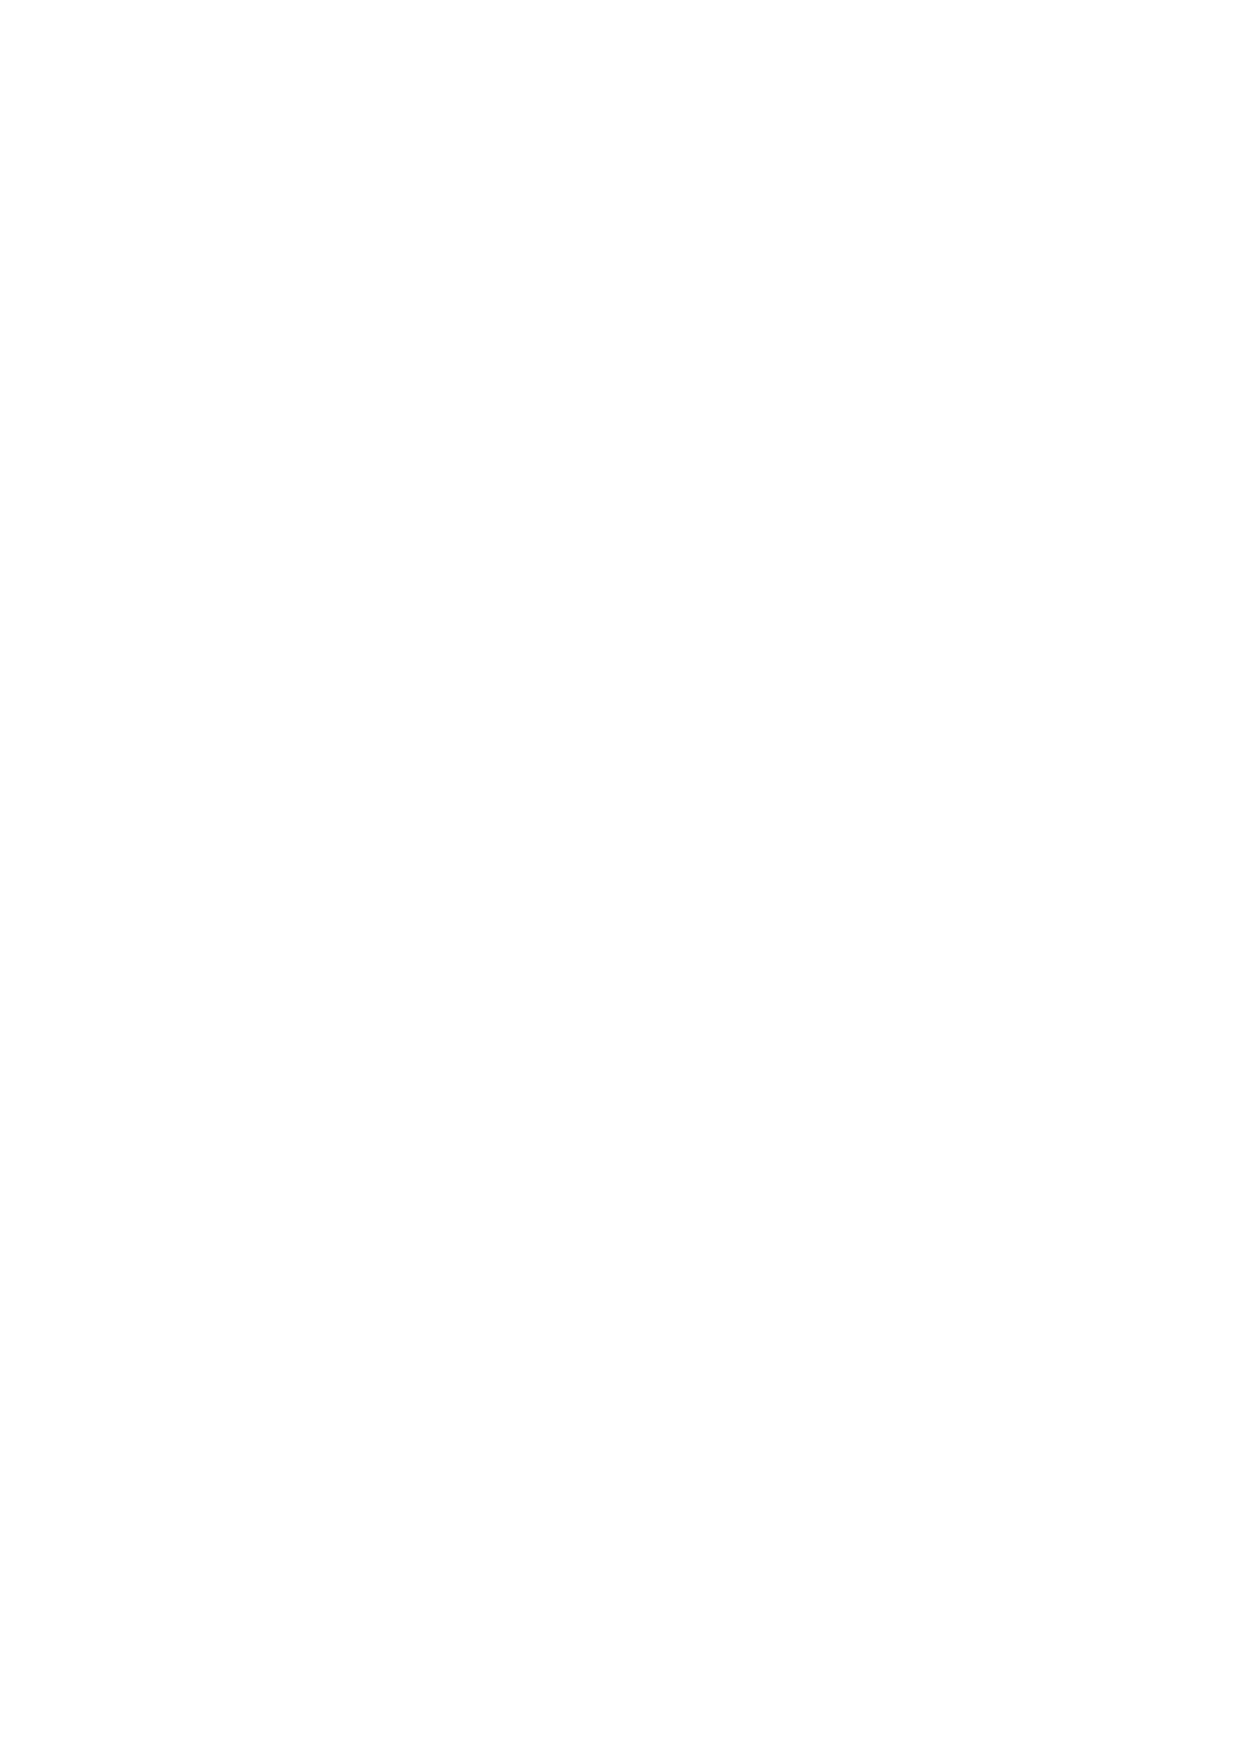
\includegraphics[scale=1.3]{immagini/DEIlogoFULL}}
    \end{figure}
    
    \vskip 3cm{
    \begin{center}\sc
        UNIVERSITY OF PADUA\\
        DEPARTMENT OF INFORMATION ENGINEERING\\
        MASTER DEGREE IN COMPUTER ENGINEERING\end{center}
		}
		
		\vskip1.2cm\begin{center}
      \rm\large\uppercase\expandafter{A.A. 2009/2010\\}
 \end{center}
    	
    \vskip 2.5cm\begin{center}
    \HRule \\[0.4cm]\LARGE\expandafter{BATCH SIZE ESTIMATE}
    \HRule \\[0.4cm]
    \end{center}
    
    \begin{flushright}\vskip4.0cm 
    \begin{tabular}{rl}
            \rm\large \uppercase{Supervisor:} &\emph{Prof. Andrea Zanella}\\
	   \rm\large \uppercase{Student:} &\emph{Marco Bettiol} \\
		\end{tabular}
     \end{flushright}
    \vfill
          \begin{center}
                  \vskip1.0cm 
                  Last Update: \today  \hspace{1mm } \currenttime
           \end{center}
    
\end{titlepage}

\newpage
%%pagina vuota
%\clearpage\null\thispagestyle{empty}\clearpage

%\setcounter{page}{1}

%\tableofcontents

\section*{Introduzione}
Un vettore $x$ di lunghezza N può essere visto come una sequenza $x_0,...,x_{N-1}$ di N numeri complessi. Si definisce $X$ \emph{trasformata discreta di Fourier (DFT, discrete Fourier transform)}  di $x$ la sequenza $X_0,...,X_{N-1}$ espressa dalla seguente relazione:
\begin{equation*}
\label{eq:def-dft}
X_k=\sum_{n=0}^{N-1}x_ne^{-\jmath\frac{2\pi}{N}kn} \quad k=0,...,N-1
\end{equation*}
La \emph{FFT} o \emph{trasformata veloce di Fourier} individua una famiglia di algoritmi in grado di calcolare la DFT in tempo $O(N \log N)$ al posto dell'usuale $O(N^{2})$ ottenibile banalmente attraverso la definizione.\\
Molti di questi algoritmi, oltre che ad essere computazionalmente efficienti, si prestano bene anche ad un'implementazione parallela.\\
In questo lavoro è stata realizzata un'implementazione del noto algoritmo di Cooley-Tukey.
\section{Algoritmo}
L'algoritmo di Cooley-Tukey prevede di calcolare la DFT del vettore $x$ attraverso il calcolo separato delle DFT delle sottosequenze di indice pari e dispari della sequenza originaria e quindi la loro ricombinazione attraverso \emph{operazioni butterlfy} tra elementi in posizione analoga delle due sottosequenze per ottenere la trasformata della originale.\\
L'immagine seguente illustra quanto appena enunciato per una sequenza di lunghezza 8
\begin{figure}[H] 
  \centering
      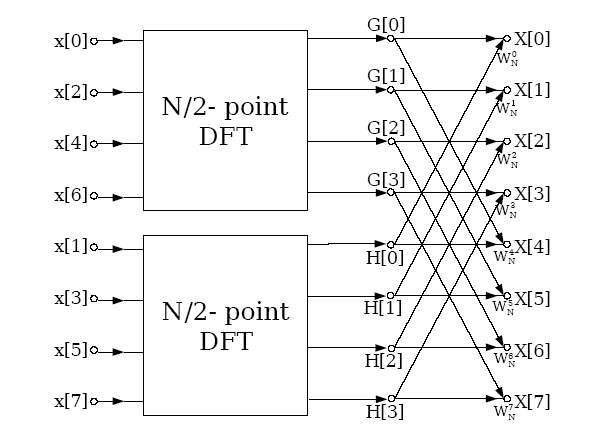
\includegraphics[width=\textwidth]{immagini/cooley-tukey}
  \caption{Ricombinazione in Cooley-Tukey per una sequenza di lunghezza 8}
\end{figure}
Questo rimescolamento dell'input iniziale, operato a ritroso fino al caso base di sequenze di lunghezza 2, permette di notare come l'algoritmo di CT sia costituito da una rete ascendente che ha come input il vettore originale rimescolato in ordine \emph{bitreversal}.
\begin{figure}[H] 
  \centering
      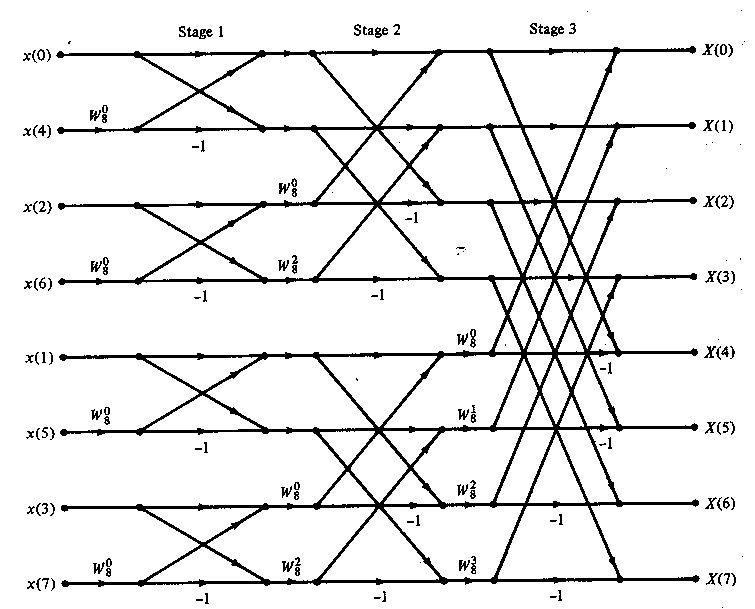
\includegraphics[width=\textwidth]{immagini/alg-asc}
  \caption{bitreversal di una sequenza di lughezza 8 e computazione su rete ascendente}
\end{figure}
Ora, considerando una sequenza di lunghezza N e avendo a disposizione P processori, è possibile dividere la sequenza iniziale in P blocchi da $\frac{N}{P}$ elementi. Il processore $i$-esimo sarà responsabile dell'$i$-esimo blocco. Notiamo come la computazione sia inizialmente priva di comunicazioni in quanto ogni processore dispone localmente dei dati da elaborare. Soltanto le ultime $\log_{2} P$ fasi richiedono infatti l'utilizzo di dati di responsabilità di un altro processore. In queste fasi che chiameremo ``esterne'' (analogamente consideriamo ``interne'' le fasi precedenti), il processore $x$, utilizzando la notazione vista a lezione, comunicherà prima con $C_{0}x$, quindi con $C_{1}x$,...
In generale, nella $j$-esima fase esterna, si avrà lo scambio dei rispettivi blocchi di responsabilità tra
$$x  \longleftrightarrow  C_{j}x \quad \textrm{per} \quad j=0,...,\log_{2} P-1 $$

\section{Implementazione}
Per prima cosa è stata sviluppata un'implementazione sequenziale iterativa dell'algoritmo di CT cercando di seguire i suggerimenti visti a lezione per quanto riguarda l'ottimizzazione del codice. I cicli (3) utilizzati per la computazione sono stati modificati in modo da essere decrescenti (es: da N-1 a 0) e ordinati in modo da elaborare il vettore dei dati in maniera contigua (posizione i, i+1, e così via) al fine di ridurre gli accessi ed utilizzare nel modo migliore RAM e soprattutto cache.\\
Particolare attenzione è stata inoltre riposta nella gestione dei \emph{twiddle factors}.\\
Per elaborare una sequenza di lunghezza N è necessario calcolare $\frac{N}{2}$ \emph{twiddle factors} ($ \omega_{N}^{0},...,\omega_{N}^{\frac{N}{2}-1}$). Tuttavia soltanto nell'ultima fase vengono utilizzati tutti i \emph{twiddle factors} mentre nelle fasi precedenti si utilizzano solo alcuni di questi (ottenibili come un sottocampionamento del vettore appena calcolato). Ad esempio nella prima fase si utilizza, banalmente, $ \omega_{N}^{0}=1$, nella seconda $ \omega_{N}^{0}$ e $\omega_{N}^{\frac{N}{4}}=-j$, nella terza $ \omega_{N}^{0}$, $\omega_{N}^{\frac{N}{8}}$, $\omega_{N}^{\frac{N}{4}}$, $\omega_{N}^{\frac{3N}{8}}$ e così via.\\
Pertanto sottocampionando progressivamente il vettore \emph{twiddle factors} mantenendo solo gli elementi in posizione dispari si è prodotto un vettore di lunghezza 2N-1 che ha in posizioni contigue i \emph{twiddle factors} opportuni che saranno impiegati in ciascun stadio. Con uno ``spreco'' di $\frac{N}{2}$ di RAM ulteriormente occupata è stato pertanto ottimizzato l'accesso in RAM/cache ai fattori di ricombinazione. Questo ha fornito un ulteriore boost prestazionale molto evidente.\\
L'implementazione sequenziale così ottenuta è stata quindi utilizzata come base di partenza per:
\begin{enumerate}
\item un algoritmo ascendente con chiamate bloccanti
\item un algoritmo ascendente con chiamate non-bloccanti
\end{enumerate}
\subsection{Sceletro generale dell'algoritmo}

Il processore con rank 0 è eletto come coordinatore del gruppo di processori e si occupa della gestione, distribuzione e raccolta dei dati elaborati.

Le fasi principali che possiamo individuare dall'algoritmo sono:
\begin{enumerate}
\item $P_{0}$ legge l'input da file o lo genera se richiesto
\item $P_{0}$ dispone l'input in bit-reversal
\item Ogni processore calcola localmente i \emph{twiddle factors} e li memorizza in un vettore
\item $P_{0}$ distribuisce a ciascun processore la porzione di input di cui è responsabile attraverso una chiamata MPI\_Scatter
\item Calcolo della FFT parallela prima nelle dimensioni interne e poi in quelle esterne
\item $P_{0}$ raccoglie i risultati attraverso un MPI\_Gather
\item $P_{0}$ scrive l'eventuale output
\end{enumerate}
 
\subsubsection{Algoritmo ascendente bloccante}
Per l'implementazione della modalità bloccante, poichè ogni processore manda dati e li riceve dallo stesso ``collega'' si è utilizzata la primitiva
\begin{verbatim}
MPI_Sendrecv(sendbuf, sendcount, sendtype, dest, sendtag, recvbuf, 
               recvcount, recvtype, source, recvtag, comm, status)
\end{verbatim} 
che prevede lo scambio mutuo di dati tra due processori.  
\subsubsection{Algoritmo ascendente non-bloccante}
Come già detto ogni processore gestisce $\frac{N}{P}$ elementi memorizzati in un vettore.\\
Denominiamo con A e B rispettivamente la prima e la seconda metà del vettore (A e B contengono quindi $\frac{N}{2P}$ elementi ciascuno). Indichiamo inoltre con A' e B' i dati provenienti dal processore ``collega''.
Per ogni stadio (completo) in cui è necessaria la comunicazione con altri processori questa avviene nel seguente modo:
\begin{enumerate}
\item Attesa per il completamento della ricezione di B' e l'invio di B
\item Aggiornamento di B
\item Invio di B e ricezione di B' 
\item Attesa per il completamento della ricezione di A' e l'invio di A
\item Aggiornamento di A
\item Invio di A e ricezione di A'  
\end{enumerate}
In questo caso le primitive utilizzate sono quelle non bloccanti, non bufferizzate
\begin{center}
\begin{verbatim}
                MPI_Isend, MPI_Irecv, MPI_Wait 
\end{verbatim} 
\end{center}
La scelta di suddividere il vettore in due metà e comunicarne prima l'una e poi l'altra è nata dall'idea di
\begin{enumerate}
\item limitare l'impatto del costo della gestione della comunicazione. Infatti tanto più sovrapposte sono calcolo e comunicazione (pacchetti scambiati piccoli) tanto più sforzo è richiesto alla macchina per la gestione dei buffer della comunicazione
\item cercare di limitare il ritardo dovuto alla comunicazione a quello dell'invio di $\frac{N}{2P}$ elementi + delay iniziale. 
\end{enumerate}

\subsection{Modalità d'uso}

Il software sviluppato funziona per
\begin{itemize}
\item $N=2^{n}$; lunghezza della sequenza da elaborare
\item $P=2^{p}$; numero di processori impiegati
\item $P<N$; quindi risulta $\frac{N}{P}\geq 2$ in modo da avere come caso base sempre operazioni tra due elementi.
\end{itemize}

\noindent Il programma prevede 2 distinte modalità di esecuzione.\\
La prima è utile per la valutazione delle performance dell'algoritmo, la seconda per l'effettivo impiego.
Consideriamo $n=\log_{2}N$
\begin{description}
\item[ Test su sequenza nota ] Il nodo $P_{0}$ genera un'input di lunghezza $2^{n}$  e quindi procede con il calcolo parallelo della sua FFT. \\ La sintassi è:
\begin{verbatim}
      ./fft-asc-* test n
\end{verbatim}
\item[ Elaborazione dell'input fornito]  $P_{0}$ legge da file l'input che dopo l'elaborazione viene salvato in un file di output
\begin{verbatim}
      ./fft-asc-* read n file_input file_output
\end{verbatim}
dove *$\in$\{sp, cp\} per richiamare rispettivamente la versione bloccante o non bloccante.
\end{description}
\subsection{Formato dei file elaborati}
Il i file sono letti/scritti con \emph{fscanf}  / \emph{fprintf}. I file devono essere costituiti da una sequenza di coppie di numeri intervallati da spazi o return. Per ciascuna coppia il primo elemento viene interpretato come parte la reale mentre il secondo come parte immaginaria dell'effettivo valore da elaborare.\\
Ad esempio:\\
\begin{center}
\fbox{\parbox[c]{2cm}{\begin{center}0 0\\ 1 0\\  2 0\\ 3 0\end{center}}} $\longleftrightarrow$\fbox{\parbox[c]{2cm}{\begin{center}0 0 1\\ 0  2 0\\ 3 0\end{center}}} $\longleftrightarrow$ \fbox{\parbox[c]{2cm}{\begin{center}$0+j0$\\$ 1+j0$\\  $2+j0$\\ $3+j0$\end{center}}} 
\end{center}


\section{Prestazioni}
\subsection{Note su FFT Sequenziale e Cache}
Durante l'implementazione dell'algoritmo è emersa la critica dipendenza tra le prestazioni ottenute dall'algoritmo FFT-DIT2 rispetto alla dimensione della cache della macchina su cui viene lanciato.\\
L'algoritmo implementato infatti, per la natura stessa degli operatori \emph{butterfly}, risulta assolutamente non-cachefriendly.\\
L'accesso in memoria non è locale: ad ogni stadio dell'algoritmo un valore dell'input viene letto/sovrascritto una ed una sola volta. Quando l'accesso ai dati non è spazialmente localizzato e la struttura di computazione è rigida la classica modalità di mapping\\
\begin{center}
\emph{cache address} $=$ \emph{memory address} modulo \emph{cache\_size} 
\end{center}
perde di efficacia. Nel nostro caso si verifica quando la distanza tra i dati da elaborare (potenza di due) è vicina alla dimensione della cache (anch'essa potenza di due).\\
Proponiamo qui di seguito i grafici sullo Cache Miss e MFlops per illustrare la drammaticità del problema.\\
In entrambi i casi le performance diminuiscono drasticamente quando la taglia del problema supera $2^{16}=65536$ per mantenersi successivamente costanti.\\ La diminuzione praticamente lineare delle performance per $N=16$ visibile in Figura \ref{Miss} è conseguenza raddoppio del numero di \emph{twiddle factor} utilizzati ad ogni passo.\\
Le performance inferiori, a parità di stage, per le istanze di taglia maggiore sono probabilmente dovute allo swap in/out dei twiddle factor il cui address mapping entra in conflitto con quello dei valori nel vettore da elaborare.\\
Una volta oltrepassata la soglia critica il Load per Miss si stabilizza sui $5,92$ più di $100$ volte peggiore rispetto agli stage in-cache. 
Analogamente per gli stage out-of-cache si hanno circa $81/60$ Mflops/s.

\begin{figure}[h!]
  \centering
      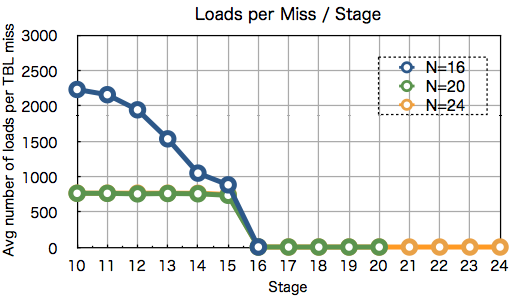
\includegraphics[width=\textwidth]{immagini/Miss}
  \caption{Caricamento di dati utili nei registri / accessi in ram. Maggiore è migliore}
\label{Miss}
\end{figure}

\begin{figure}[h!] 
  \centering
      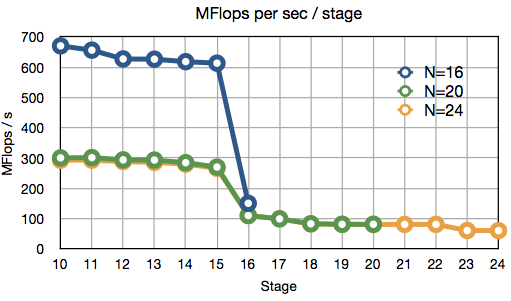
\includegraphics[width=\textwidth]{immagini/Mflops}
  \caption{Potenza di calcolo sfruttata. Maggiore è migliore}
\label{MFlops}
\end{figure}
Notiamo come $N=20$ e $N=24$ abbiano esattamente lo stesso andamento.
\end{document}